\documentclass[a4paper, twoside, openany]{book}
\usepackage[fontset=windows, heading=true, zihao=-4]{ctex} % 提供中文支持,使用中易字体(宋体、楷体、黑体、仿宋)、包含页眉、基础字号为小四
\ctexset{
chapter/number = \arabic{chapter}, % 设置章节标题序号为阿拉伯数字
section/format += \Large\bfseries\raggedright, % 设置节标题样式
}
\usepackage[utf8]{inputenc} % 设置文档使用 UTF-8 编码方案编码
\usepackage[T1]{fontenc} % 设置字体编码
\usepackage[colorlinks, citecolor=black, filecolor=black, linkcolor=black, urlcolor=black]{hyperref} % 提供超链接功能,并设置链接颜色为黑色
\usepackage[style=apa, backend=biber]{biblatex} % 提供参考文献处理功能,引用格式为 APA 格式,后端引擎设为 biber(可以支持非英文字符)
\addbibresource{Chapters/xbib.bib} % 参考文献数据库
\usepackage[toc, page, title, titletoc, header]{appendix} % 提供与附录标题相关的一些功能,添加“附录”字样,添加到目录
\usepackage{makeidx} % 提供建立索引功能
\makeindex % 建立索引
\usepackage[totoc]{idxlayout} % 提供与索引有关的功能,添加索引到目录
\usepackage[top=2.54cm,bottom=2.54cm,left=3.17cm,right=3.17cm]{geometry} % 提供页边距设置功能,设置上下页边距为 2.54 cm,左右页边距为 3.17 cm
\usepackage{fancyhdr} % 提供设置页眉页脚功能
\pagestyle{fancy}
\fancyhead{} % 清空页眉
\fancyfoot{} % 清空页脚
\fancyhead[CE,CO]{华东师范大学博士学位论文} % 设置奇数页和偶数页均居中输出“华东师范大学博士学位论文”
\fancyfoot[LE,RO]{\thepage} % 设置奇数页居左、偶数页居右输出页码
\newcommand{\notefig}[2][1]{\parbox{#1\linewidth}{\flushleft \footnotesize \textit{注:}#2}} % 自定义 \notefig 命令用于输出图注
\newcommand{\notetable}[2][1]{\parbox{#1\linewidth}{\flushleft \footnotesize \textit{注:}#2}} % 自定义 \notetable 命令用于输出表注


\usepackage{amsmath} % 提供与数学公式相关的功能
\usepackage{amsfonts} % 提供数学相关字体
\usepackage{mathptmx} % 使用 Times Roman 字体
\usepackage{gensymb} % 提供常用符号支持,例如摄氏度符号,千分号等
\usepackage{graphicx} % 提供与图像有关的增强功能
\usepackage{booktabs} % 提供三线表中上下边界加粗的横线
\usepackage{caption} % 提供图表标题与交叉引用的位置矫正功能
\usepackage[flushleft]{threeparttable} % 提供表注环境
\usepackage{rotating} % 提供整页图表功能
\usepackage{siunitx} % 提供与单位相关的一些功能
\usepackage{tikz} % 提供强大的绘图功能
\usetikzlibrary{positioning} % 使用 TikZ 提供的方位功能
\tikzset{mynode/.style={draw, text width=1in, align=center}} % 定义 mynode 样式(含有文字的方框)
\usepackage{tabularray} % 提供 tblr 表格环境




\begin{document}

\frontmatter
\pagenumbering{alph} % 使用字母页码
\pdfbookmark{标题页}{} % 添加标题页书签
\begin{titlepage}
\noindent
{2222 届研究生博士学位论文\\
\makebox[2.2cm][s]{分类号:} \underline{\makebox[3cm]{}}\hfill
\makebox[2.2cm][s]{学校代码:} \underline{\makebox[3cm]{10269}}\\
\makebox[2.2cm][s]{密级:} \underline{\makebox[3cm]{}}\hfill
\makebox[2.2cm][s]{学号:} \underline{\makebox[3cm]{22222222222}}\\
}

\vspace{2cm}
\begin{center}
    
\includegraphics[width=0.8\textwidth]{Pictures/Pages/ecnu.png}\\
    {\large East China Normal University}

    \vspace{0.5cm}
    {\large 博士学位论文\par
    DOCTORAL DISSERTATION}

    \vspace{2cm}
    {\huge\centering
    \makebox[3.6cm][s]{论文题目:}
    \underline{\makebox[7.8cm]{填充文本填充文本}}\par
    \makebox[3.6cm][s]{}
    \underline{\makebox[7.8cm]{填充文本填充文本}}\par
    }

    \vfill
    {\large\centering\parskip1ex
    \makebox[3.6cm][s]{院系:} \underline{\makebox[7.8cm]{填充文本}}\par
    \makebox[3.6cm][s]{专业:} \underline{\makebox[7.8cm]{填充文本}}\par
    \makebox[3.6cm][s]{研究方向:} \underline{\makebox[7.8cm]{填充文本}}\par
    \makebox[3.6cm][s]{学位申请人:} \underline{\makebox[7.8cm]{填充文本}}\par
    \makebox[3.6cm][s]{指导教师:} \underline{\makebox[7.8cm]{填充文本}}\par
    }

    \vspace{1.5cm}
    {\large 2222 年 2 月}
\end{center}
\end{titlepage}
\newpage

%%%%%%%%%%%%%%%%%%%%%%%%%%%%%%%%%%%%%%%%%%%%%%%%%%%%%%%%%%%%%%%%%%%%

\thispagestyle{empty}
{\noindent Dissertation for Doctoral Degree in 2222\\
\makebox[2.2cm]{} \hfill \makebox[2.8cm][s]{University code:} \underline{\makebox[3cm]{10269}}\\
\makebox[2.2cm]{} \hfill \makebox[2cm][s]{Student ID:} \underline{\makebox[3cm]{22222222222}}\\
}

\vspace{3cm}
\begin{center}
    {\large East China Normal University}

    \vspace{3cm}
    {\huge\centering
    \makebox[2cm][s]{Title:} \underline{\makebox[11cm]{The Quick Brown Fox Jumps}}\par
    \makebox[2cm][s]{} \underline{\makebox[11cm]{The Quick Brown Fox Jumps}}\par
    \makebox[2cm][s]{} \underline{\makebox[11cm]{The Quick Brown Fox}}\par
    }

    \vfill
    {\centering\parskip1.5ex
    \makebox[3.8cm]{Department/School:} \underline{\makebox[9.2cm]{The Quick Brown Fox}}\par
    \makebox[3.8cm]{Major:} \underline{\makebox[9.2cm]{The Quick Brown Fox}}\par
    \makebox[3.8cm]{Research direction:} \underline{\makebox[9.2cm]{The Quick Brown Fox}}\par
    \makebox[3.8cm]{Candidate:} \underline{\makebox[9.2cm]{The Quick Brown Fox}}\par
    \makebox[3.8cm]{Supervisor:} \underline{\makebox[9.2cm]{The Quick Brown Fox}}\par
    }

    \vspace{2cm}
    {\large Feb, 2222}
\end{center}

\newpage

\thispagestyle{empty}
{\centerline{\Large \bf 华东师范大学学位论文原创性声明}

\vspace{0.5cm}
郑重声明:本人呈交的学位论文《违反社会规范的意图对第三方干预的影响》,是在华东师范大学攻读硕士/博士(请勾选)学位期间,在导师的指导下进行的研究工作及取得的研究成果。除文中已经注明引用的内容外,本论文不包含其他个人已经发表或撰写过的研究成果。对本文的研究做出重要贡献的个人和集体,均已在文中作了明确说明并表示谢意。

\vspace{0.5cm}
{\bf 作者签名} \hfill {\bf 日期}\makebox[1.5cm]{}年\makebox[1cm]{}月\makebox[1cm]{}日

\vfill
\centerline{\Large \bf 华东师范大学学位论文著作权使用声明}

\vspace{0.5cm}
《违反社会规范的意图对第三方干预的影响》系本人在华东师范大学攻读学位期间在导师指导下完成的硕士/博士(请勾选)学位论文,本论文的著作权归本人所有。本人同意华东师范大学根据相关规定保留和使用此学位论文,并向主管部门和学校指定的相关机构送交学位论文的印刷版和电子版;允许学位论文进入华东师范大学图书馆及数据库被查阅、借阅;同意学校将学位论文加入全国博士、硕士学位论文共建单位数据库进行检索,将学位论文的标题和摘要汇编出版,采用影印、缩印或者其它方式合理复制学位论文。

本学位论文属于(请勾选)\\
\indent(\makebox[0.5cm]{})1.经华东师范大学相关部门审查核定的“内部”或“涉密”学位论文*,于\makebox[0.8cm]{} 年 \makebox[0.5cm]{} 月 \makebox[0.5cm]{} 日解密,解密后适用上述授权。\\
\indent(\makebox[0.5cm]{})2.不保密,适用上述授权。

\vspace{0.5cm}
{\bf 导师签名} \hfill {\bf 作者签名} \makebox[4cm]{}

\vspace{0.5cm}
\hfill {\bf 日期}\makebox[1.5cm]{}年\makebox[1cm]{}月\makebox[1cm]{}日

\vfill
* “涉密”学位论文应是已经华东师范大学学位管理办公室或保密委员会审定过的学位论文(需附获批的《华东师范大学研究生申请学位论文“涉密”审批表》方为有效),未经上述部门审定的学位论文均为公开学位论文。此声明栏不填写的,默认为公开学位论文,均适用上述授权)。
}

\newpage

\thispagestyle{empty}
{\centerline{\large 此页请附答辩材料中答辩决议【复印件】}}

% 
\includegraphics[width=0.8\textwidth]{Pictures/Pages/ecnu.png}\\
\newpage

%%%%%%%%%%%%%%%%%%%%%%%%%%%%%%%%%%%%%%%%%%%%%%%%%

\thispagestyle{empty}
{\centerline{\Large \bf \underline{\makebox[2cm]{}}博士学位论文导师指导小组同意答辩的确认声明}

\vspace{0.5cm}
本人已认真阅读此篇学位论文,该论文已达到申请博士学位论文答辩水平。\parskip3ex \par
\makebox[1cm]{} \hfill 指导小组成员签名:\makebox[5cm]{}\par
\makebox[1cm]{} \hfill \makebox[1.5cm]{}年\makebox[1cm]{}月\makebox[1cm]{}日

\vfill
本人已认真阅读此篇学位论文,该论文已达到申请博士学位论文答辩水平。\par
\makebox[1cm]{} \hfill 指导小组成员签名:\makebox[5cm]{}\par
\makebox[1cm]{} \hfill \makebox[1.5cm]{}年\makebox[1cm]{}月\makebox[1cm]{}日

\vfill
本人已认真阅读此篇学位论文,该论文已达到申请博士学位论文答辩水平。\par
\makebox[1cm]{} \hfill 指导小组成员签名:\makebox[5cm]{}\par
\makebox[1cm]{} \hfill \makebox[1.5cm]{}年\makebox[1cm]{}月\makebox[1cm]{}日

\vfill
本人已认真阅读此篇学位论文,该论文已达到申请博士学位论文答辩水平。\par
\makebox[1cm]{} \hfill 指导小组成员签名:\makebox[5cm]{}\par
\makebox[1cm]{} \hfill \makebox[1.5cm]{}年\makebox[1cm]{}月\makebox[1cm]{}日

\vfill
本人已认真阅读此篇学位论文,该论文已达到申请博士学位论文答辩水平。\par
\makebox[1cm]{} \hfill 指导小组成员签名:\makebox[5cm]{}\par
\makebox[1cm]{} \hfill \makebox[1.5cm]{}年\makebox[1cm]{}月\makebox[1cm]{}日
}

\newpage

%%%%%%%%%%%%%%%%%%%%%%%%%%%%%%%%%%%%%%%%%%%%%%%%%

\thispagestyle{empty}
{\centerline{\large 此页请附答辩材料2:学位论文导师评阅及同意答辩意见表【复印件】}}

% 
\includegraphics[width=0.8\textwidth]{Pictures/Pages/ecnu.png}\\
\newpage

\thispagestyle{empty}
{\centerline{\Large \bf \underline{\makebox[2cm]{}}博士学位论文开题小组成员签名单}

\vspace{1cm}
\begin{centering}
\begin{tblr}{
  colspec = {X[c,m]X[c,m]X[c,m]X[c,m]X[c,m]},
  stretch = 0,
  rowsep = 8pt,
  hlines = {0.5pt},
  vlines = {0.5pt},
  rows   = {ht = \baselineskip}
}
      姓名 & 职称 & 单位 & 签名 \\
           &      &      &      \\
           &      &      &      \\
           &      &      &      \\
           &      &      &      \\
           &      &      &      \\
\end{tblr}
\end{centering}
}

\newpage

%%%%%%%%%%%%%%%%%%%%%%%%%%%%%%%%%%%%%%%%%%%%%%%%%

\thispagestyle{empty}
{\centerline{\Large \bf \underline{\makebox[2cm]{}}博士学位论文预答辩小组成员签名单}

\vspace{1cm}
\begin{centering}
\begin{tblr}{
  colspec = {X[c,m]X[c,m]X[c,m]X[c,m]X[c,m]},
  stretch = 0,
  rowsep = 8pt,
  hlines = {0.5pt},
  vlines = {0.5pt},
  rows   = {ht = \baselineskip}
}
      姓名 & 职称 & 单位 & 签名 \\
           &      &      &      \\
           &      &      &      \\
           &      &      &      \\
           &      &      &      \\
           &      &      &      \\
\end{tblr}
\end{centering}
}

\newpage

%%%%%%%%%%%%%%%%%%%%%%%%%%%%%%%%%%%%%%%%%%%%%%%%%

\thispagestyle{empty}
{\centerline{\Large \bf \underline{\makebox[2cm]{}}博士学位论文答辩委员会专家签名单}

\vspace{1cm}
\begin{centering}
\begin{tblr}{
  colspec = {X[c,m]X[c,m]X[c,m]X[c,m]X[c,m]},
  stretch = 0,
  rowsep = 8pt,
  hlines = {0.5pt},
  vlines = {0.5pt},
  rows   = {ht = \baselineskip}
}
      姓名 & 职称 & 单位 & 签名 & 备注 \\
           &      &      &      & 主席 \\
           &      &      &      & \\
           &      &      &      & \\
           &      &      &      & \\
           &      &      &      & \\
\end{tblr}
\end{centering}
}

\newpage

\pagenumbering{roman} % 使用小写罗马数字页码
\thispagestyle{plain}
\centerline{\Large \bf 中文摘要}

\vspace{0.5cm}
填充文本填充文本填充文本填充文本填充文本填充文本填充文本填充文本填充文本填充文本填充文本填充文本填充文本填充文本填充文本填充文本填充文本填充文本。

填充文本填充文本填充文本填充文本填充文本填充文本填充文本填充文本填充文本填充文本填充文本填充文本填充文本填充文本填充文本填充文本填充文本填充文本。

\vspace{0.5cm}
{\noindent \bf 关键词:}填充文本、填充文本

%%%%%%%%%%%%%%%%%%%%%%%%%%%%%%%%%%%%%%%%%%%%%%%%%%%%%%%%%%%%%
\newpage
\thispagestyle{plain}
% \vspace{1cm}
\centerline{\Large \bf Abstract}

\vspace{0.5cm}
The quick brown fox jumps over the lazy dog. The quick brown fox jumps over the lazy dog. The quick brown fox jumps over the lazy dog. The quick brown fox jumps over the lazy dog. The quick brown fox jumps over the lazy dog. 


\vspace{0.5cm}
{\noindent \bf Keywords:} The quick, brown fox
\newpage

\pdfbookmark{\contentsname}{toc} % 添加目录页书签
\tableofcontents % 输出目录

\mainmatter
\chapter{绪论}

填充文本填充文本填充文本填充文本填充文本填充文本填充文本填充文本填充文本填充文本填充文本填充文本填充文本填充文本填充文本填充文本填充文本填充文本。

\section{填充文本}

填充文本填充文本填充文本填充文本填充文本填充文本填充文本填充文本填充文本填充文本填充文本填充文本填充文本填充文本填充文本填充文本填充文本填充文本。

\subsection{填充文本}

填充文本填充文本填充文本填充文本填充文本填充文本填充文本填充文本填充文本填充文本填充文本填充文本填充文本填充文本填充文本填充文本填充文本填充文本。

填充文本填充文本填充文本填充文本填充文本填充文本填充文本填充文本填充文本填充文本填充文本填充文本填充文本填充文本填充文本填充文本填充文本填充文本。

\subsection{填充文本}

填充文本填充文本填充文本填充文本填充文本填充文本填充文本填充文本填充文本填充文本填充文本填充文本填充文本填充文本填充文本填充文本填充文本填充文本。

\section{填充文本}

填充文本填充文本填充文本填充文本填充文本填充文本填充文本填充文本填充文本填充文本填充文本填充文本填充文本填充文本填充文本填充文本填充文本填充文本。

\chapter{问题提出和研究方案}

\section{填充文本}

填充文本填充文本填充文本填充文本填充文本填充文本填充文本填充文本填充文本填充文本填充文本填充文本填充文本填充文本填充文本填充文本填充文本填充文本。

填充文本填充文本填充文本填充文本填充文本填充文本填充文本填充文本填充文本填充文本填充文本填充文本填充文本填充文本填充文本填充文本填充文本填充文本。

\section{填充文本}

填充文本填充文本填充文本填充文本填充文本填充文本填充文本填充文本填充文本填充文本填充文本填充文本填充文本填充文本填充文本填充文本填充文本填充文本。

填充文本填充文本填充文本填充文本填充文本填充文本填充文本填充文本填充文本填充文本填充文本填充文本填充文本填充文本填充文本填充文本填充文本填充文本。

\chapter{研究一:填充文本}

填充文本填充文本填充文本填充文本填充文本填充文本填充文本填充文本填充文本填充文本填充文本填充文本填充文本填充文本填充文本填充文本填充文本填充文本。

\section{实验一:填充文本}

填充文本填充文本填充文本填充文本填充文本填充文本填充文本填充文本填充文本填充文本填充文本填充文本填充文本填充文本填充文本填充文本填充文本填充文本。图表引用如:见图 \ref{plot_random_points}。

\begin{figure}[htbp]
    \centering
    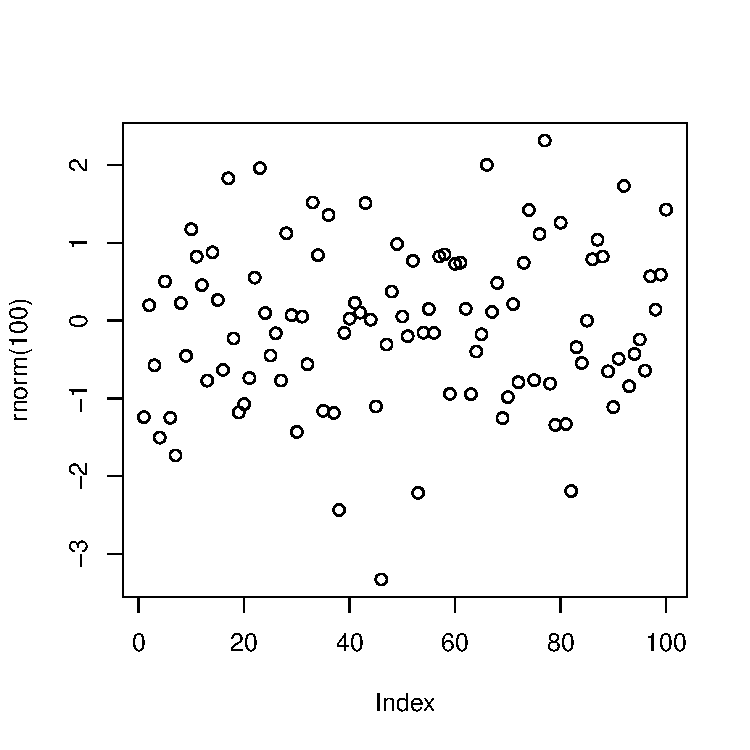
\includegraphics[width=0.5\linewidth]{Pictures/Exp1/plot_random_points.pdf}
    \caption{100 个正态分布的随机数}
    \label{plot_random_points}
    \notefig{100 个正态分布的随机数。填充文本填充文本填充文本填充文本填充文本填充文本填充文本填充文本填充文本填充文本填充文本填充文本填充文本填充文本填充文本填充文本填充文本填充文本。}
\end{figure}

填充文本填充文本填充文本填充文本填充文本填充文本填充文本填充文本填充文本填充文本填充文本填充文本填充文本填充文本填充文本填充文本填充文本填充文本。表格引用如:见表 \ref{table_fit}。

\begin{table}
    \centering
    \begin{threeparttable}
        \caption{填充文本填充文本}
        \label{table_fit}
        \begin{tabular*}{0.9\textwidth}{l @{\extracolsep{\fill}} r r c r r @{\extracolsep{0cm}} @{} l}
            \toprule
            & \multicolumn{1}{c}{$b$} & \multicolumn{1}{c}{SE} & \multicolumn{1}{c}{95\% CI} & \multicolumn{1}{c}{df} & \multicolumn{2}{c}{$t$} \\
            \midrule
            填充文本      &  1.11  &  1.11  & $(1.11, 2.22)$ &  11  &  11.11  &  $^{***}$  \\
            填充文本  &  1.11  &  1.11  & $(1.11, 2.22)$ &  11  &  11.11  &  $^{**}$  \\
            填充文本  &  1.11  &  1.11  & $(1.11, 2.22)$ &  11  &  11.11  &  $^{*}$  \\
            填充文本  &  1.11  &  1.11  & $(1.11, 2.22)$ &  11  &  11.11  &  $^{\dagger}$\\
            \bottomrule
        \end{tabular*}
        \notetable{填充文本填充文本填充文本填充文本填充文本填充文本填充文本填充文本填充文本填充文本填充文本填充文本填充文本填充文本填充文本填充文本填充文本填充文本。\\
        $^{***} p < 0.001; \quad ^{**} p < 0.01; \quad ^{*} p < 0.05; \quad ^{\dagger} p < 0.1$}
    \end{threeparttable}
\end{table}

填充文本填充文本填充文本填充文本填充文本填充文本填充文本填充文本填充文本填充文本填充文本填充文本填充文本填充文本填充文本填充文本填充文本填充文本。

\begin{sidewaysfigure}
    \centering
    \begin{tikzpicture}
        \node at(0, 0) [mynode] (x) {起始点};
        \node at(7, 0) [mynode] (m1) {中间点一};
        \node at(13, 1.5) [mynode] (m2) {中间点二};
        \node at(13, -1.5) [mynode] (m3) {中间点三};
        \node at(19, 0) [mynode] (y) {终点};

        \draw[-latex] (x.east) -- node[above, font=\footnotesize, align=left]{$a_1 = 1.11^{*}$ \\ $a_2 = 1.11^{*}$} (m1.west);

        \draw[-latex] (m1.east) -- (m2.west);
        \draw (10, 1.3) node[font=\footnotesize]{$m_1 = -1.11^{*}$};
        \draw[-latex] (m1.east) -- (m3.west);
        \draw (10, -1.3) node[font=\footnotesize]{$m_2 = -1.11^{*}$};

        \draw[-latex] (m2.east) -- (y.west);
        \draw (16, 1.2) node[font=\footnotesize]{$b_1 = 1.11^{*}$};
        \draw[-latex, dashed] (m3.east) -- (y.west);
        \draw (16, -1.2) node[font=\footnotesize]{$b_2 = 1.11$};

        \draw[-latex] (x.south) -- (0, -3) -- (19, -3) -- (y.south);
        \draw (7, -2.2) node[font=\footnotesize, align=left]{$c'_1 = 1.11^{*}$ \\ $c'_2 = 1.11^{*}$};
        \draw (7, -3.8) node[font=\footnotesize, align=left]{$c_1 = 1.11^{*}$ \\ $c_2 = 1.11^{*}$};
    \end{tikzpicture}
    \caption{TikZ 绘图示例}
    \label{plot_flow}
    \notefig{填充文本填充文本填充文本填充文本填充文本填充文本填充文本填充文本填充文本填充文本填充文本填充文本填充文本填充文本填充文本填充文本填充文本填充文本。}
\end{sidewaysfigure}




\section{实验二:填充文本}

填充文本填充文本填充文本填充文本填充文本填充文本填充文本填充文本填充文本填充文本填充文本填充文本填充文本填充文本填充文本填充文本填充文本填充文本。


\chapter{研究二:填充文本}

填充文本填充文本填充文本填充文本填充文本填充文本填充文本填充文本填充文本填充文本填充文本填充文本填充文本填充文本填充文本填充文本填充文本填充文本。

\section{实验三:填充文本}

填充文本填充文本填充文本填充文本填充文本填充文本填充文本填充文本填充文本填充文本填充文本填充文本填充文本填充文本填充文本填充文本填充文本填充文本。

\section{实验四:填充文本}

填充文本填充文本填充文本填充文本填充文本填充文本填充文本填充文本填充文本填充文本填充文本填充文本填充文本填充文本填充文本填充文本填充文本填充文本。


\chapter{总讨论}

填充文本填充文本填充文本填充文本填充文本填充文本填充文本填充文本填充文本填充文本填充文本填充文本填充文本填充文本填充文本填充文本填充文本填充文本。

\chapter{总结}

填充文本填充文本填充文本填充文本填充文本填充文本填充文本填充文本填充文本填充文本填充文本填充文本填充文本填充文本填充文本填充文本填充文本填充文本。

\nocite{*} % 输出参考文献数据库中所有文献
\printbibliography[title={参考文献}] % 参考文献标题
\addcontentsline{toc}{chapter}{参考文献} % 添加参考文献到目录
\appendix % 停止章节编码,使用附录编码
\chapter{附录}

\section{使用说明}

本模板主要面向心院的同学,不需要超出普通使用 \LaTeX 的知识,适合初学者和喜欢 DIY 的同学。模板包含了学校对学位论文所要求的全部结构,但是在一些细节上并没有完全遵照规定(见第 \pageref{后记} 页)。模板中 \texttt{main.tex} 是主要框架文件,其他都是辅助文件,编译时只需要编译主要框架文件即可。

\section{编译步骤}

本模板使用 XeLaTeX 引擎编译。正常情况下您只需要在文件所在目录执行 \verb`xelatex main.tex` 命令即可输出文档。如果您使用的是 MiKTex 发行版,那么您可以在 TeXworks 编辑器里选择排版引擎后点击 
\includegraphics{Pictures/Appendix/pic_xelatx.png} 按钮。

如果您更新了参考文献,那么需要按照以下步骤编译:

\begin{enumerate}
    \item 使用 XeLaTeX 引擎编译 
\includegraphics{Pictures/Appendix/pic_xelatx.png}
    \item 使用 Biber 引擎编译 
\includegraphics{Pictures/Appendix/pic_biber.png}
    \item 使用 XeLaTeX 引擎重新编译 
\includegraphics{Pictures/Appendix/pic_xelatx.png}
    \item 再次使用 XeLaTeX 引擎编译 
\includegraphics{Pictures/Appendix/pic_xelatx.png}
\end{enumerate}

第一步是为了生成辅助文件,第二步依据参考文献数据库 \texttt{xbib.bib} 更新 \texttt{.bbl} 文件,第三步排版文档,第四步更新文档的交叉引用。

如果您更新了索引,那么您需要在第二步把 Biber 引擎换为 MakeIndex 引擎 
\includegraphics{Pictures/Appendix/pic_makeindex.png},更新 \texttt{.idx} 文件。

对于不需要频繁更新参考文献的文档,TeXworks 提供了一个快捷的排版引擎组合 
\includegraphics{Pictures/Appendix/pic_xelate_makeindex.png},可以一键输出包含索引的文档。


\backmatter
\include{Chapters/Pages/Pages_简介和成果}
\include{Chapters/Pages/Pages_后记}
% \printindex

\end{document}
